\documentclass[french,t]{beamer}
\usetheme{Madrid}
\usepackage{graphicx}
\usepackage{tikz}
\usepackage{fancyhdr}
\usetikzlibrary{automata, positioning, arrows}


\title{Stanks.io}
\subtitle{encadré par M.Leprêtre et M.Dubois}
\author{Hey Monika !}
\institute{ULCO}
\titlegraphic{%
	
\includegraphics[width=.25\linewidth]{images/Logo_ULCO}
}
\date{25 Juin 2020}

\begin{document}
	\begin{frame}[plain, noframenumbering]
		\maketitle
	\end{frame}
	\begin{frame}
		\frametitle{Répartition des tâches}
		\begin{block}{Rôles}
			\begin{description}
				\item<1->[Pecqueux Théo :] Contrôles du jeu
				\item<2->[Huyghes Antoine :] Git master, interface graphique
				\item<3->[Villette Vincent :] Communications réseau
				\item<4->[Skibinski Pierre :] Chef de projet , moteur de jeu.
			\end{description}
		\end{block}
	\end{frame}
	\begin{frame}
		\frametitle{Présentation du jeu}
		\begin{columns}
			\begin{column}{0.5\textwidth}
				Contrôles (manette)
				\begin{figure}
					\centering
					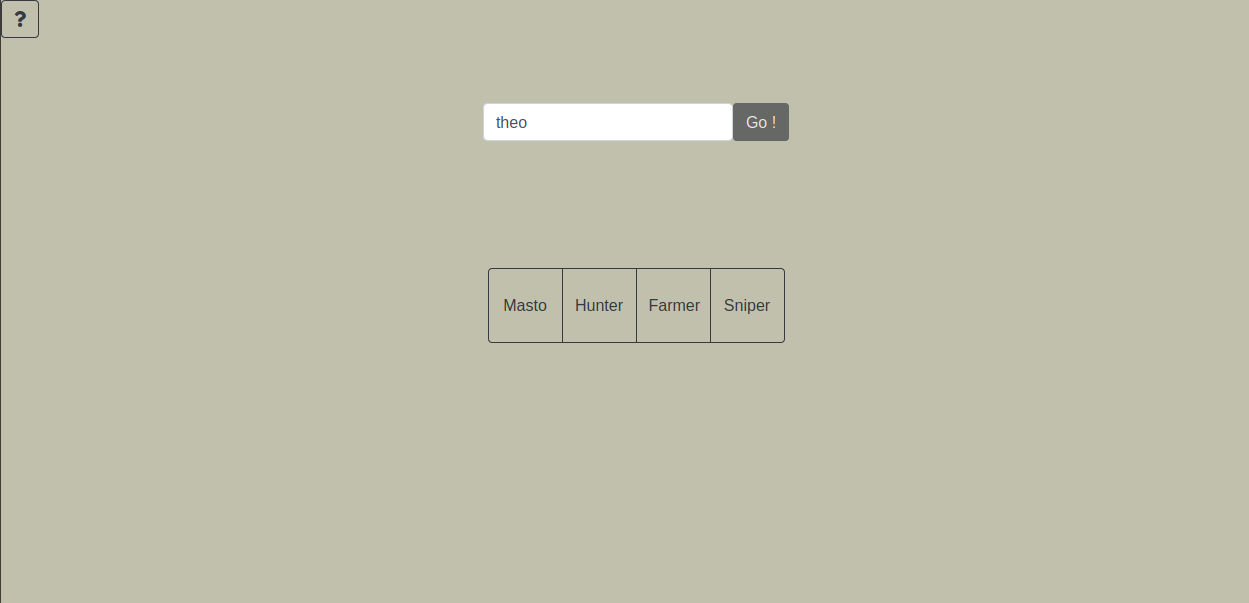
\includegraphics[height=2.5cm]{images/name}
				\end{figure}
				\begin{figure}
					\centering
					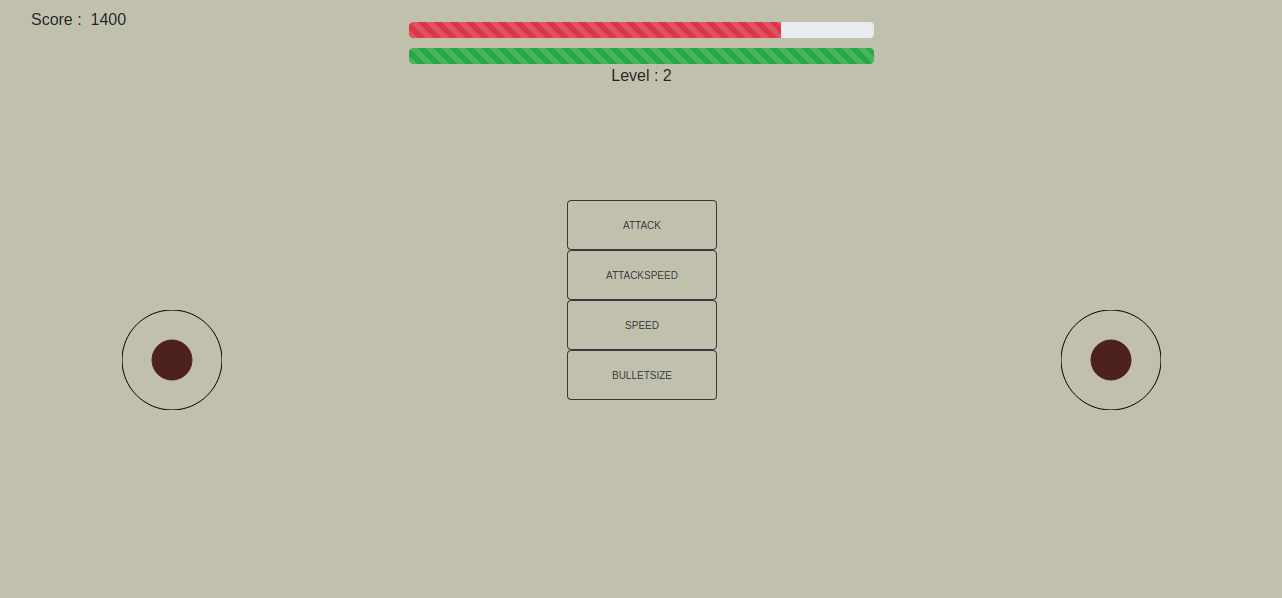
\includegraphics[height=2.5cm]{images/controls}
				\end{figure}
			\end{column}
			\pause
			\begin{column}{0.5\textwidth}
				Écran
				\begin{figure}
					\centering
					\includegraphics[height=2.5cm]{images/fullPlayers}
				\end{figure}
				\begin{figure}
					\centering
					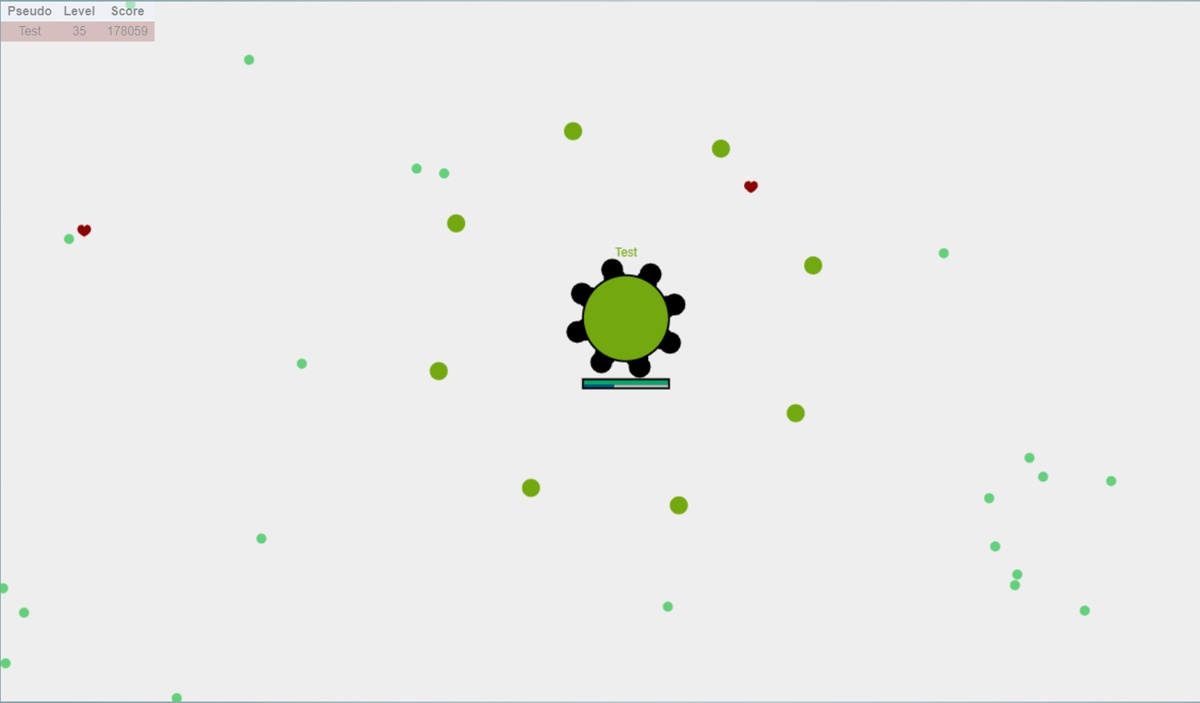
\includegraphics[height=2.5cm]{images/tank-upgrade}
				\end{figure}
			\end{column}
		\end{columns}
			
	\end{frame}
	\begin{frame}
		\frametitle{Organisation}
		\begin{block}{Git}
			\begin{itemize}
				\item 5 branches: 1 master + 1 par contributeurs
				\item Jalons et issues qui couvrent les besoins fonctionnels
			\end{itemize}
		\end{block}
	\pause
	\begin{block}{Equipe}
	\begin{itemize}
		\item Utilisation d'une méthodologie agile: Scrum
		\item Utilisation de Discord
		\item Briefing à 9h
		\item Bilan de la journée à 16h
	\end{itemize}
\end{block}
	\end{frame}
	\begin{frame}
		\frametitle{Indicateurs de productivité}
		\begin{block}{Statistiques du projet}
			\begin{description}
				\centering
				\item<1->[Lignes de codes :] 1328
				\item<2->[Tests unitaires (CICD) :] 70 \% du moteur du jeu
				\item<3->[Nombre de jalons :] 4
				\item<4->[Nombre d'issues :] 20
				\item<5->[Commits :] 600
			\end{description}
		\end{block}
	\end{frame}
	\begin{frame}
		\frametitle{Bilan}
		\begin{block}{Prise de recul}
			\begin{itemize}
				\item Début: Manque d'organisation pas assez de gestion de projet
				\item Commit seulement quand une fonctionnalité est implémenté
			\end{itemize}
		\end{block}
		\pause
		\begin{exampleblock}{Point positif}
			\begin{itemize}
				\item Expérience
				\item Entente au sein du groupe
				\item Gestion des branches
				\item Projet captivant
			\end{itemize}
		\end{exampleblock}
	\end{frame}
	\begin{frame}[plain, noframenumbering]
		\vspace*{\fill}
		\begin{block}{}
		\frametitle{}
			\centering
			Merci de votre attention. Avez-vous des questions?
		\end{block}
		\vspace*{\fill}
	\end{frame}

\end{document}